
%-------------------------------------------------------------------
%	PACKAGES AND THEMES
%-------------------------------------------------------------------

%\documentclass{beamer}
\documentclass[handout]{beamer}

\mode<presentation> {
\usetheme{CambridgeUS}
}
\usecolortheme{seahorse}
\setbeamertemplate{itemize items}[circle]
\beamertemplatenavigationsymbolsempty

\makeatletter
\setbeamertemplate{footline}
{%
  \leavevmode%
  \hbox{%
   \begin{beamercolorbox}[wd=.25\paperwidth,ht=2.25ex,dp=1ex,center]{title in head/foot}%
    \usebeamerfont{title in head/foot}\insertshorttitle
  \end{beamercolorbox}%
  \begin{beamercolorbox}[wd=.50\paperwidth,ht=2.25ex,dp=1ex,center]{author in head/foot}%
    \usebeamerfont{author in head/foot}\insertshortauthor\expandafter\ifblank\expandafter{\beamer@shortinstitute}{}{~~(\insertshortinstitute)}
  \end{beamercolorbox}%
 
  \begin{beamercolorbox}[wd=.25\paperwidth,ht=2.25ex,dp=1ex,leftskip=2ex,rightskip=2ex,sep=0pt]{date in head/foot}%
    \hfill%
    \usebeamerfont{date in head/foot}%
    \insertshortdate{}%
    \hfill%
    \usebeamercolor[fg]{page number in head/foot}%
    \usebeamerfont{page number in head/foot}%
    \usebeamertemplate{page number in head/foot}%
  \end{beamercolorbox}}%
  \vskip0pt%
}
\makeatother

\usepackage{graphicx} % Allows including images
\usepackage{booktabs} % Allows the use of \toprule, \midrule and \bottomrule in tables
\usepackage{amsmath}
\usepackage{multirow}
\usepackage{array}
\usepackage{neuralnetwork}
\usepackage{booktabs,caption}
\usepackage[flushleft]{threeparttable}
\usepackage{tikz}
\usetikzlibrary{positioning,chains}
\usepackage{caption}
\setbeamertemplate{caption}[numbered]
\usepackage{yhmath}
\usepackage{wrapfig}


\newcommand{\Sum} [2] {\the\numexpr #1 + #2 \relax \\}
%-------------------------------------------------------------------
%	TITLE PAGE
%-------------------------------------------------------------------

\title[Forecasting Volatility]{Forecasting Volatility} % The short title appears at the bottom of every slide, the full title is only on the title page

\author{Multivariate Statistical Methods and Applications} % Your name
\institute[] % Your institution as it will appear on the bottom of every slide, may be shorthand to save space
{
\medskip
\text{Anatol Sluchych} % Your email address
}

\date{December 14, 2023} % Date, can be changed to a custom date

\begin{document}

\begin{frame}
\titlepage % Print the title page as the first slide
\end{frame}
%-------------------------------------------------------------------
\begin{frame}
\frametitle{Outline} 
\tableofcontents % Throughout your presentation, if you choose to use \section{} and \subsection{} commands, these will automatically be printed on this slide as an overview of your presentation
\end{frame}

%-------------------------------------------------------------------
%	PRESENTATION SLIDES
%-------------------------------------------------------------------

%-------------------------------------------------------------------
\section{Why Forecasting Volatility?} % Sections can be created in order to organize your presentation into discrete blocks, all sections and subsections are automatically printed in the table of contents as an overview of the talk
%-------------------------------------------------------------------


\begin{frame}
\frametitle{Forecasting Stock Return Volatility}

Applications:
\begin{itemize}
\item risk management
\pause
\item derivative pricing
\pause
\item devising trading strategies
\end{itemize}

\vspace{15mm}
\pause

Realized volatility (RV) as proxy for unobserved volatility:
$\mathrm{RV}_{i, t}^{(h)}:=  \displaystyle\sum_{s=t-h+1}^t r_{i, s}^2 $, for period 
$[t-h, t]$

\end{frame}

%------------------------------------------------
\begin{frame}
\frametitle{Model Comparison}

\begin{table}
\begin{threeparttable}
\caption{\label{table01}Models' out-of-sample performance (QLIKE loss function).}
\begin{tabular}{|llll|}
\hline \hline 
\multirow{2}{*}{Model \hspace{23mm}} & \multicolumn{3}{c|}{Intraday  Volatility Frequency} \\ 
 & \multicolumn{1}{l}{10-min} \hspace{6mm} & \multicolumn{1}{l}{30-min} \hspace{6mm} & 60-min \\ \hline \hline  
HAR & \multicolumn{1}{l}{0.197} & \multicolumn{1}{l}{0.187} & 0.186 \\ 
OLS & \multicolumn{1}{l}{0.186} & \multicolumn{1}{l}{0.187} & 0.186\\ 
LASSO & \multicolumn{1}{l}{0.191} & \multicolumn{1}{l}{0.187} & 0.186\\
XGBoost & \multicolumn{1}{l}{0.177} & \multicolumn{1}{l}{0.173} & 0.173 \\ 
NN (MLP) & \multicolumn{1}{l}{{\color[HTML]{009901} 0.171}} & \multicolumn{1}{l}{{\color[HTML]{009901} 0.171}} &  0.172\\ 
NN (LSTM) & \multicolumn{1}{l}{0.174} & \multicolumn{1}{l}{{\color[HTML]{009901} 0.171}} &  {\color[HTML]{009901} 0.171} \\ \hline
\end{tabular}
    \begin{tablenotes}
      {\scriptsize
      \item Source: Zhang et al. (2023). MPL: 3 hidden layers, LSTM: 2 hidden layers.}
    \end{tablenotes}
\end{threeparttable}
\end{table}

\begin{itemize}
\item neural networks (multilayer perceptron and long short-term memory) yield superior forecasts


\end{itemize}
\end{frame}

%------------------------------------------------
\section{Gentle Introduction to Neural Networks}
%------------------------------------------------

\begin{frame}
\frametitle{(Artificial) Neural Networks}

\begin{columns}[onlytextwidth]
\begin{column}{.6\textwidth}
\begin{itemize}
    \item inspired by how human brains work
    \item universal function approximators
\end{itemize}
\end{column}
\begin{column}{.4\textwidth}
\begin{center}
\begin{figure}[h]
\caption{Human neural network}
\centering
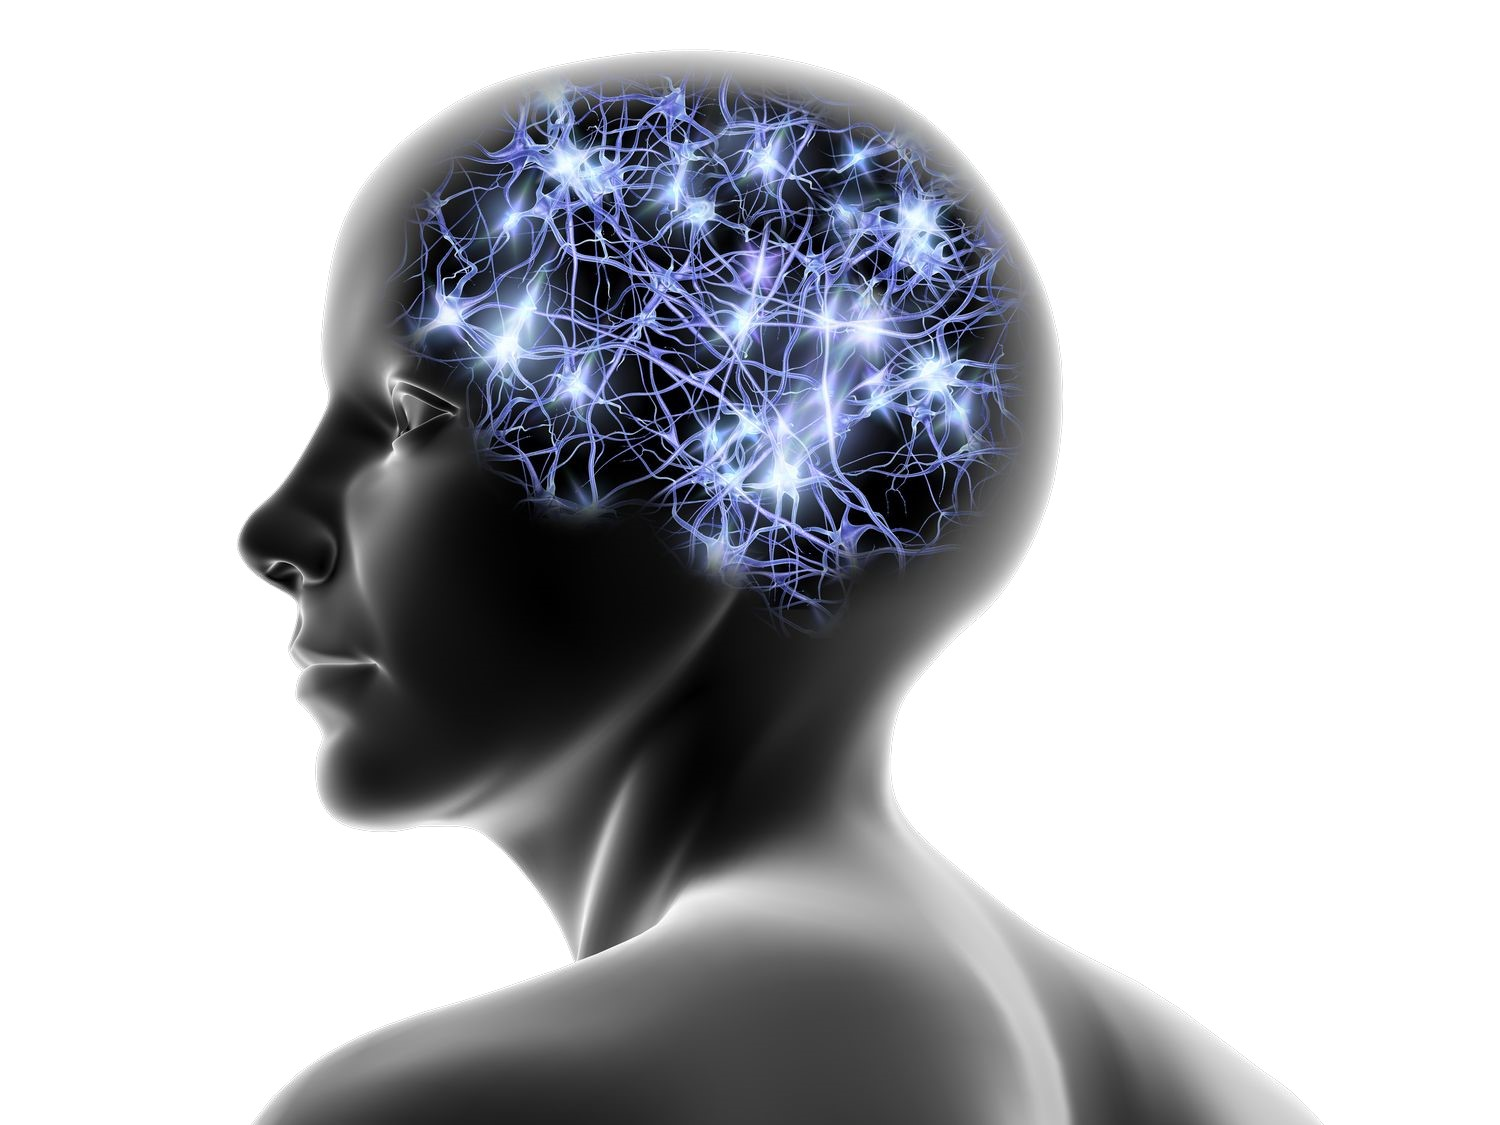
\includegraphics[scale=0.12]{pics/brain.jpeg}
\begin{minipage}{0.65\textwidth} % choose width suitably
{\scriptsize \hspace{3mm} Source: Getty Images \par}
\end{minipage}
\end{figure}
\end{center}
\end{column}        
\end{columns}


\begin{itemize}
    \pause
    \item $y_i = x_i^T \beta + \varepsilon_i$ \hspace{15mm} (linear regression)
    \vspace{2mm}
    \pause
    \item $y_i = g(x_i^T \beta) + \varepsilon_i$
    \pause
    \item $\displaystyle y_i=\sum_{j=1}^rg_j(x_i^T \beta_j) + \varepsilon_i$ \hspace{2mm} (projection pursuit regression)
\end{itemize}




\end{frame}
%------------------------------------------------

\begin{frame}
\frametitle{Single Hidden Layer Neural Network}
\begin{align*}
\begin{neuralnetwork}[height=2]
\newcommand{\x}[2]{$RV_{t-#2}$}
\newcommand{\y}[2]{$g(RV)$}
\newcommand{\h}[2]{$A_#2$}
\newcommand{\w}[4]{$\omega_{#2#4}$}
\newcommand{\B}[4]{$\beta_#2$}
\newcommand{\naught}[4]{}
\newcommand{\nodetexty}[2]{$\widehat{RV}_{t}$}
\setdefaultlinklabel{\w}
\inputlayer[count=2, bias=false, title=Input\\layer, text=\x]
\hiddenlayer[count=2, bias=false, title=Hidden\\layer, text=\h]
\foreach \n in {1,...,2}{
    \foreach \m in {1,2}{
        \link[style={}, labelpos=near start, from layer=0, from node=\n, to layer=1, to node=\m]
    }
}
\outputlayer[count=1, title=Output\\layer,  text=\y] 
\setdefaultlinklabel{\B} \linklayers
\outputlayer[count=1, nodeclass={input neuron}, title=\nodetexclear, text=\nodetexty]     \setdefaultlinklabel{\naught} \linklayers
\end{neuralnetwork}
\end{align*}

\begin{itemize}
    \pause
    \item activations: $A_1 = g(\omega_{11}RV_{t-1} + \omega_{21}RV_{t-2} + b_1)$, \\
    \pause
    \hspace{20mm}$A_2 = g(\omega_{12}RV_{t-1} + \omega_{22}RV_{t-2} + b_2)$
    \pause
    \item $g(z)$: \textit{nonlinear} activation function
    \pause
    \item $\widehat{RV}_t = g(RV) =  g(\beta_1A_1 + \beta_2A_2 + a_1)  \\
    \pause
    \hspace{13.7mm} \scriptsize{  =  g  (\beta_1g(\omega_{11}RV_{t-1} + \omega_{21}RV_{t-2} + b_1) + \beta_2g(\omega_{12}RV_{t-1} + \omega_{22}RV_{t-2} + b_2) + a_1})$
    
\end{itemize}
\end{frame}


\begin{frame}
\frametitle{Activation Functions}
\begin{center}
\begin{figure}[h]
\caption{Common activation functions}
\centering
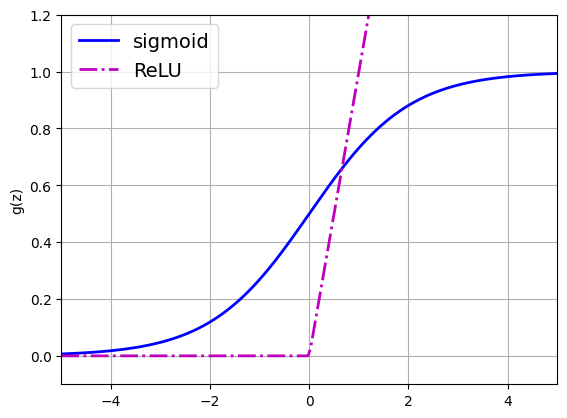
\includegraphics[scale=0.5]{pics/activations.png}
\end{figure}
\end{center}


\begin{itemize}
    \item sigmoid: $g(z) = \frac{1} {1 + e^{-z}}, \pause \hspace{3mm} e.g. \hspace{1mm} $A_1 = \frac{1} {1 + e^{-(\omega_{11}RV_{t-1} + \omega_{21}RV_{t-2} + b_1)}} $
    \pause
    \item ReLU (\textit{rectifi￱ed linear unit}): $g(z) = max(0, z)$
\end{itemize}
\end{frame}




%------------------------------------------------
\begin{frame}
\frametitle{Training}

\begin{center}
\begin{figure}[h]
\caption{Gradient descent}
\centering
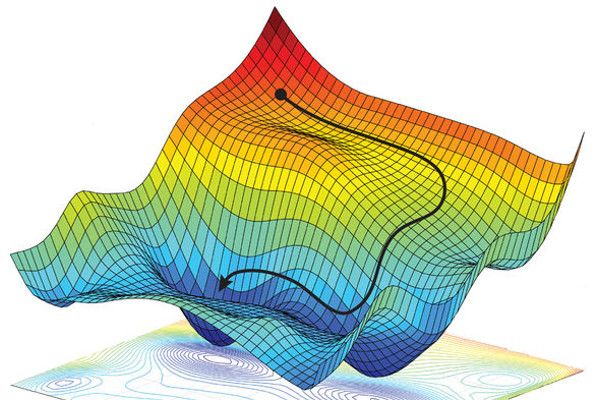
\includegraphics[scale=0.5]{pics/gradient_descent.jpg}
\begin{minipage}{0.65\textwidth} % choose width suitably
{\scriptsize \hspace{20mm} Source: Amini et al. (2018) \par}
\end{minipage}
\end{figure}
\end{center}


\begin{itemize}
    \item weights and biases: random starting values near zero 
    \pause
    \item backpropagation (through gradient descent) until  minimum of loss function is reached
    \pause
    \item training epoch: one sweep through the entire training set
\end{itemize}
\end{frame}

\begin{frame}
\frametitle{Multilayer Neural Network}
Multilayer perceptron: \textit{uni-directional} feedforward NN
\vspace{10mm}

\begin{neuralnetwork}[height=5]
\newcommand{\x}[2]{$RV_{t-#2}$}
\newcommand{\y}[2]{$g(RV)$}
\newcommand{\hone}[2]{$A^{(1)}_#2$}
\newcommand{\htwo}[2]{$A^{(2)}_#2$}
\newcommand{\w}[4]{$w_{#2#4}$}
\newcommand{\B}[4]{$\beta_#2$}
\newcommand{\naught}[4]{}
\newcommand{\nodetexty}[2]{$\widehat{RV}_t$}
\setdefaultlinklabel{\naught}
\inputlayer[count=4, bias=false, title=Input\\layer, text=\x]
\hiddenlayer[count=5, bias=false, title=Hidden\\layer 1, text=\hone]
\linklayers
\hiddenlayer[count=4, bias=false, title=Hidden\\layer 2, text=\htwo]
\linklayers
\outputlayer[count=1, title=Output\\layer,  text=\y] 
\linklayers
\outputlayer[count=1, nodeclass={input neuron}, title=\nodetexclear, text=\nodetexty]  
\linklayers
\end{neuralnetwork}
\end{frame}



\begin{frame}
\frametitle{Recurrent Neural Networks}

\begin{tikzpicture}[item/.style={circle,draw,thick,align=center},
itemc/.style={item,on chain,join}, scale=0.8]
 \begin{scope}[start chain=going right,nodes=itemc,every
 join/.style={-latex,very thick},local bounding box=chain]
 \path node (A1) {$A_1$} node (A2) {$A_2$} node (A3) {$A_3$} node[xshift=2em] (AT)
 {$A_T$};
 \end{scope}
 \node[left=1em of chain,scale=2] (eq) {$=$};
 \node[left=2em of eq,item] (AF) {$A_t$};
 \path (AF.west) ++ (-1em,2em) coordinate (aux);
 \draw[very thick,-latex,rounded corners, red] (AF.east)  -| ++ (1em,2em) -- (aux)  
 |-   node[left, pos=.3] {U} (AF.west);


 \foreach \X in {1,2,3} 
 {\draw[very thick,-latex] (A\X.north) -- ++ (0,2em)
 node[above,item,fill=gray!10] (h\X)   {$\widehat{RV}_{\Sum {\X} {1}}$};
 \draw[very thick,latex-] (A\X.south) -- ++ (0,-2em)
 node[below,item,fill=gray!10] (x\X) {$RV_\X$};}

\draw[very thick,-latex] (AT.north) -- ++ (0,2em)
 node[above,item,fill=gray!10]  (hT)   {$\widehat{RV}_{\tiny{T+1}}$};
 \draw[very thick,latex-] (AT.south) -- ++ (0,-2em)
 node[below,item,fill=gray!10] (xT) {$RV_{T}$};

 \draw[white,line width=0.8ex] (AF.north) -- ++ (0,1.9em);
 \draw[very thick,-latex]  (AF.north) -- ++  (0,2em) 
 node[above,item,fill=gray!10] {$\widehat{RV}_{t+1}$};
 \draw[very thick,latex-] (AF.south) -- ++ (0,-2em) 
 node[below,item,fill=gray!10]  {$RV_t$};
 \path (x3) -- (xT) node[midway,scale=2,font=\bfseries] {\dots};
\end{tikzpicture}


\begin{itemize}
    \item \textit{bi-directional} NN
    \item feedback loops: $ \displaystyle A_{t k}=g(b_k+\sum_{i=1}^N w_{k i} RV_{t i}+\sum_{s=1}^K u_{k s} A_{t-1, s})$
    \pause
    \item previous steps remembered
    \pause
    \item vanishing gradient problem
\end{itemize}

\end{frame}

\begin{frame}{Long Short-Term Memory}
\begin{itemize}
    \item subtype of RNN
    \pause
    \item tackles vanishing gradient problem
\end{itemize}

\vspace{10mm}

\pause
LSTM cell:
\begin{itemize}
    \item adds new information (input gate) 
    \pause
    \item forgets irrelevant information (forget gate)
    \pause
    \item passes updated information (output gate)
\end{itemize}

\end{frame}

\begin{frame}
\frametitle{Pros \& Cons}
Pros:
\begin{itemize}
\item better performance
\pause
\item capture complex non-linearities and interactions 
\pause
\item no assumption on data generating process needed
\pause
\end{itemize}

\vspace{5mm}

Cons:
\begin{itemize}
\item require big data sets
\pause
\item require hyperparameter tuning
\pause
\item harder to interpret and present ("black box")
\end{itemize}
\end{frame}

%------------------------------------------------
\section{Outlook}
%------------------------------------------------

\begin{frame}
\frametitle{Outlook}
\begin{itemize}
    \item realized volatility forecasts: random walk vs NN 
    \item intraday data: Refinitiv Datastream 
\end{itemize}
\end{frame}
%------------------------------------------------

\begin{frame}[allowframebreaks]
\frametitle{References}
\footnotesize{
\begin{thebibliography}{99} % Beamer does not support BibTeX so references must be inserted manually as below

\bibitem[Amini, 2018]{p1} Amini, Alexander, Ava Soleimany, Sertac Karaman, and Daniela Rus (2018).
\newblock  Spatial Uncertainty Sampling for End-to-End Control.
\newblock \emph{arXiv preprint arXiv:1805.04829}.


\bibitem[Bucci, 2020]{p1} Bucci, Andrea (2020).
\newblock Realized Volatility Forecasting with Neural Networks.
\newblock \emph{Journal of Financial Econometrics 18}, 502-531.


\bibitem[Hastie, 2009]{p1} Hastie, Trevor, Robert Tibshirani, Jerome H. Friedman, and Jerome H. Friedman (2009).
\newblock  The Elements of Statistical Learning: Data Mining, Inference, and Prediction.
\newblock \emph{Springer Science \& Business Media}.


\bibitem[James, 2021]{p1} James, Gareth, Daniela Witten, Trevor  Hastie, and Robert Tibshirani (2021).
\newblock  An Introduction to Statistical Learning: with Applications in R (Second Edition).
\newblock \emph{Springer Science \& Business Media}.


\bibitem[Murphy, 2022]{p1} Murphy, Kevin P. (2022).
\newblock  Probabilistic Machine Learning: An Introduction.
\newblock \emph{MIT Press}.


\bibitem[Zhang, 2023]{p1} Zhang,  Chao, Yihuang Zhang, Mihai Cucuringu, and Zhongmin Qian (2023).
\newblock Volatility Forecasting with Machine Learning and Intraday Commonality.
\newblock \emph{Journal of Financial Econometrics}, forthcoming.

\end{thebibliography}
}
\end{frame}


%------------------------------------------------

\end{document}


\begin{frame}
\frametitle{Model Comparison}
\begin{itemize}
\item data: top 93 stocks of S\&P 500
\pause
\item period: July 1, 2011 to June 30, 2021
\pause
\item pooled past intraday and daily RVs to forecast daily RVs:
\small
\mathrm{RV}_{i, t+1}^{(d)}=F_i\left(\mathrm{RV}_{i, t}^{(h)}, \ldots, \mathrm{RV}_{i, t-(p-1) b}^{(h)}, \mathrm{RV}_{i, t-1}^{(d)}, \ldots, \mathrm{RV}_{i, t-(p-1)}^{(d)} ; \theta\right)+\epsilon_{i, t+1}$
\normalsize
\item QLIKE loss function for comparison (Patton and
Sheppard 2009)
\pause
\item pooled data of all stocks and a proxy for overall market volatility
\pause
\item  rolling window estimation based on normalized observations in the last 21 days
\end{itemize}
\end{frame}

\bibitem[Engle, 2012]{p1} Engle, Robert F., and Magdalena E. Sokalska. 2012.
\newblock Forecasting Intraday Volatility in the US
Equity Market: Multiplicative Component GARCH.
\newblock \emph{Journal of Financial Econometrics} 10: 54–83.

\begin{neuralnetwork}[height=2, layerspacing=20mm] 
\newcommand{\x}[2]{$RV_#2$}
\newcommand{\y}[2]{$f(RV)$}
\newcommand{\hone}[2]{$A^{(1)}_#2$}
\newcommand{\htwo}[2]{$A^{(2)}_#2$}
\newcommand{\w}[4]{$w_{#2#4}$}
\newcommand{\B}[4]{$\beta_#2$}
\newcommand{\recurrence}[4]{$Recurrence$}
\newcommand{\naught}[4]{}
\newcommand{\nodetexty}[2]{$\widehat{RV}_5$}
\setdefaultlinklabel{\naught}
\inputlayer[count=4, bias=false, title=, text=\x]
\hiddenlayer[count=2, bias=false, title=, text=\hone]
\linklayers
\hiddenlayer[count=2, bias=false, title=, text=\htwo]

\foreach \n in {1,...,2}{
    \foreach \m in {1,2}{
        \link[style={}, labelpos=near start, from layer=1, from node=\n, to layer=2, to node=\m]
    }
}


\link[style={very thick, dotted, draw=magenta!60}, labelpos=near end, from layer=2, from node=1, to layer=1, to node=1]


\setdefaultlinklabel{\naught}
\outputlayer[count=1, title=,  text=\y] 
\linklayers
\outputlayer[count=1, nodeclass={input neuron}, title=\nodetexclear, text=\nodetexty]  
\linklayers
\end{neuralnetwork}